\section*{3. Chignolin CLN025: extending the atlas}
The second case uses the CC BY 4.0 \emph{Chignolin Simulations} deposit
\cite{chignolin}. Its full dataset comprises 3,744 adaptive-sampling
trajectories of nominal duration 50 ns (187.2 $\mu$s aggregate), generated
with ACEMD, CHARMM22*, TIP3P water and a 350 K Langevin thermostat.
For a bounded, reproducible prototype, we select the first 128 non-hidden
XTC files in archive order. These contain 63,999 frames: 127 runs have
500 frames and one has 499. The selected nominal aggregate duration is
6.4 $\mu$s; it is neither a continuous trajectory nor an unbiased ensemble.

\textbf{Coordinates and chart.}
Ten C$\alpha$ positions are converted from \AA\ to nm, centered, and rigidly
aligned to the first recorded frame by a proper Kabsch rotation.
Neighboring C$\alpha$ distances are checked to lie in $(0.3,0.5)$ nm.
Define geometric, equal-site-weight observables
\[
 R_g(X)=\sqrt{\frac1{10}\sum_{a=1}^{10}\|X_a-\bar X\|^2},
 \qquad d_{\rm ee}(X)=\|X_{10}-X_1\|,\qquad
 q(X)=(R_g,d_{\rm ee})\in\R_{\ge0}^2.
\]
These observables do not require alignment, although consistent alignment
is needed to place molecular shapes in the scene.
The observed coordinate range, padded by 0.01 nm, is mapped linearly to a
$30\times30$ visual chart. A $30\times30$ histogram is Gaussian-smoothed
at 0.85 bins with reflecting boundaries. The displayed score
$E_{\rm occ}(q)=-\log[\widehat p(q)/\widehat p_{\max}]$ is descriptive
negative log occupancy, \emph{not} an equilibrium free energy.

\begin{figure}[H]\centering
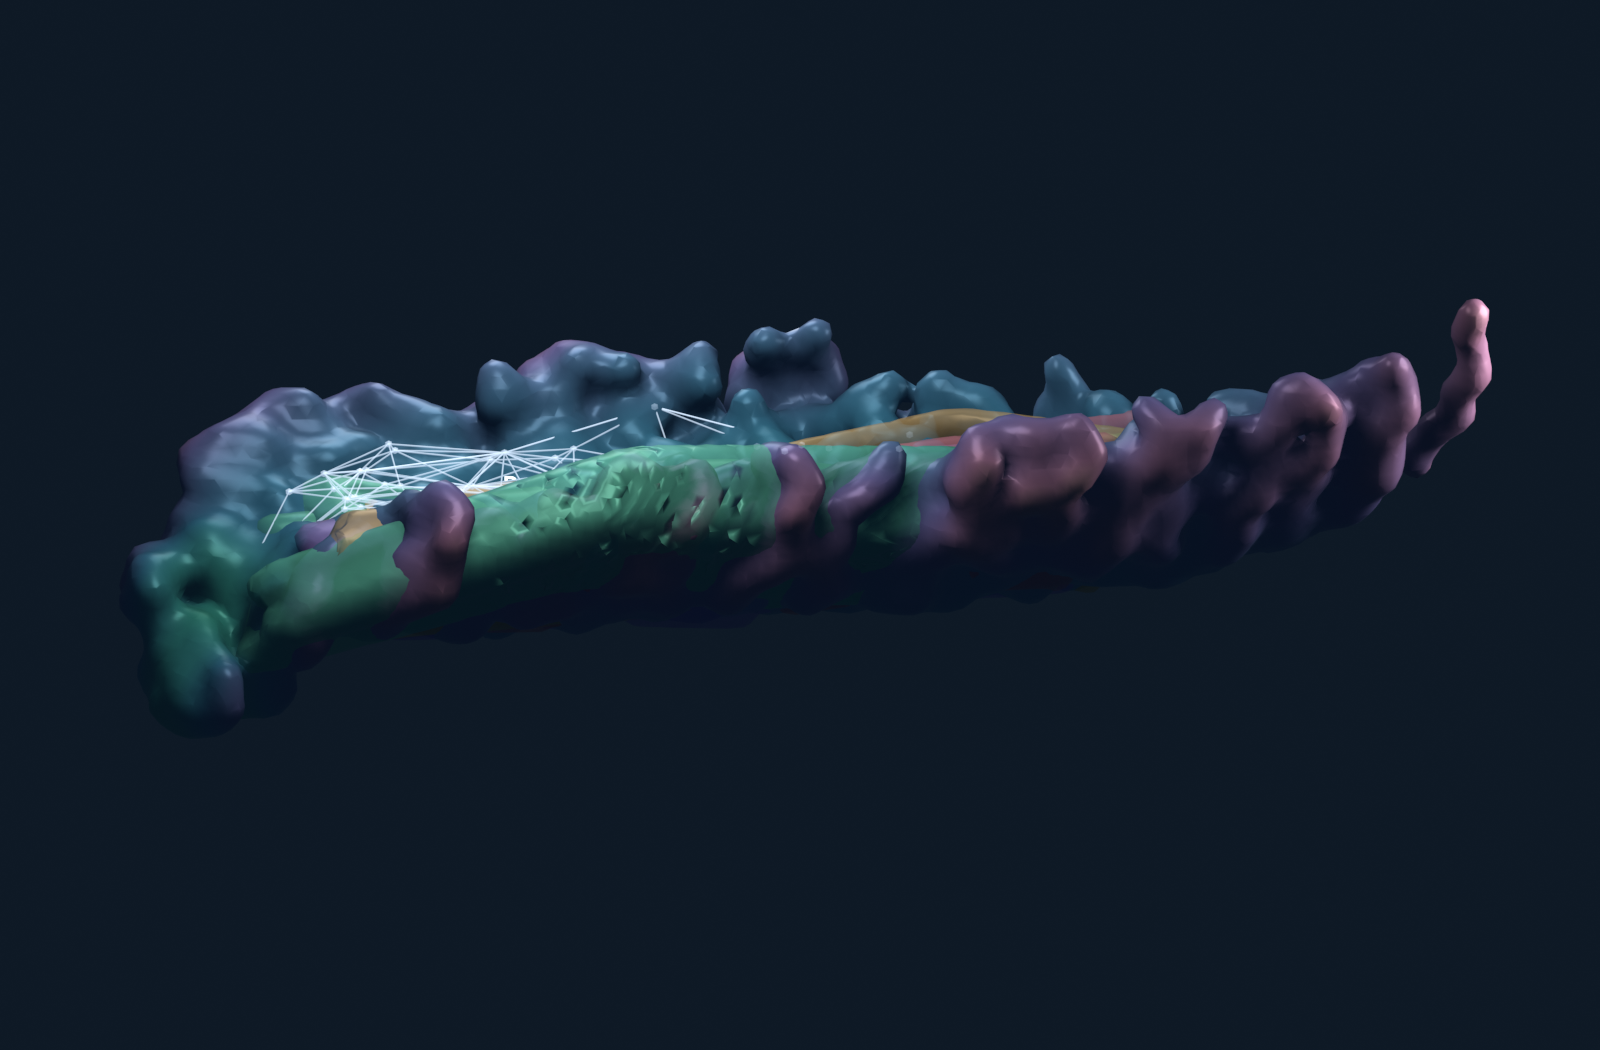
\includegraphics[width=.88\linewidth]{figures/chignolin-landscape-nerve.png}
\caption{\textbf{The CLN025 molecular landscape and overlap nerve.}
Ten-site backbone geometries generate the terrain and deforming pathway
envelopes. Silver lines show inclusions in the overlap face poset.
Horizontal axes encode $R_g$ and $d_{\rm ee}$; height combines
$1.3E_{\rm occ}$ with molecular relief. This is a visualization of the
selected adaptive sample, not a folding free-energy surface.}
\end{figure}

\newpage
\section*{Chignolin transitions and comparison}
Four $k$-means centers are fitted to every fifth observation in standardized
$(R_g,d_{\rm ee})$ coordinates, using seed 42 and 50 iterations.
Centers are ordered by increasing $R_g$ and labeled A--D.
A frame lies in a core when its nearest-center distance is at most 0.42.
The last visited core labels intervening observations. The first 129
pre-core observations are excluded; label memory resets at each run boundary.
There are 6,979 observed core-to-core passages and twelve directed route types.
These clusters are descriptive geometric states, not validated metastable
folding macrostates.

\begin{center}\small
\begin{tabular}{lrr}
\toprule Quantity & Alanine dipeptide & CLN025 subset\\\midrule
Recorded frames & 750,000 & 63,999\\
Independent runs & 3 & 128\\
Temperature & 300 K & 350 K\\
Displayed molecular sites & 10 heavy atoms & 10 C$\alpha$ sites\\
Core-to-core passages & 73,145 & 6,979\\
Observed route types & 10 & 12\\
Overlap nerve objects & 91 & 97\\
Strict inclusion arrows & 282 & 342\\
Overlap 2-simplices & 204 & 264\\
Composable generator pairs & 25 & 36\\\bottomrule
\end{tabular}
\end{center}
Counts compare software constructions, not rates or equivalent dynamical
complexity. Sampling, temperature, molecular resolution and state definitions differ.

\textbf{A finite overlap nerve.}
Fourteen farthest-point centers in the rescaled chart define radius-5.2
Euclidean balls. Every fifth observation witnesses common membership.
As for alanine, the face-poset nerve is formed from the witnessed
2-skeleton. This chart metric is a declared visualization choice;
it is not a physical distance between protein conformations.

\textbf{Pathways and skins.}
Each route uses an actual within-run passage nearest its route's median
duration in frames. At most 80 recorded conformations are retained, and
96 linearly interpolated samples define its envelope. C$\alpha$ coordinates
are magnified by 2.3 visual units/nm; Gaussians have width 0.43, grid spacing
0.30, threshold 0.65, and 0.45-voxel smoothing. The same bounded material
warp as alanine supplies twelve position/normal targets.

\begin{figure}[H]\centering
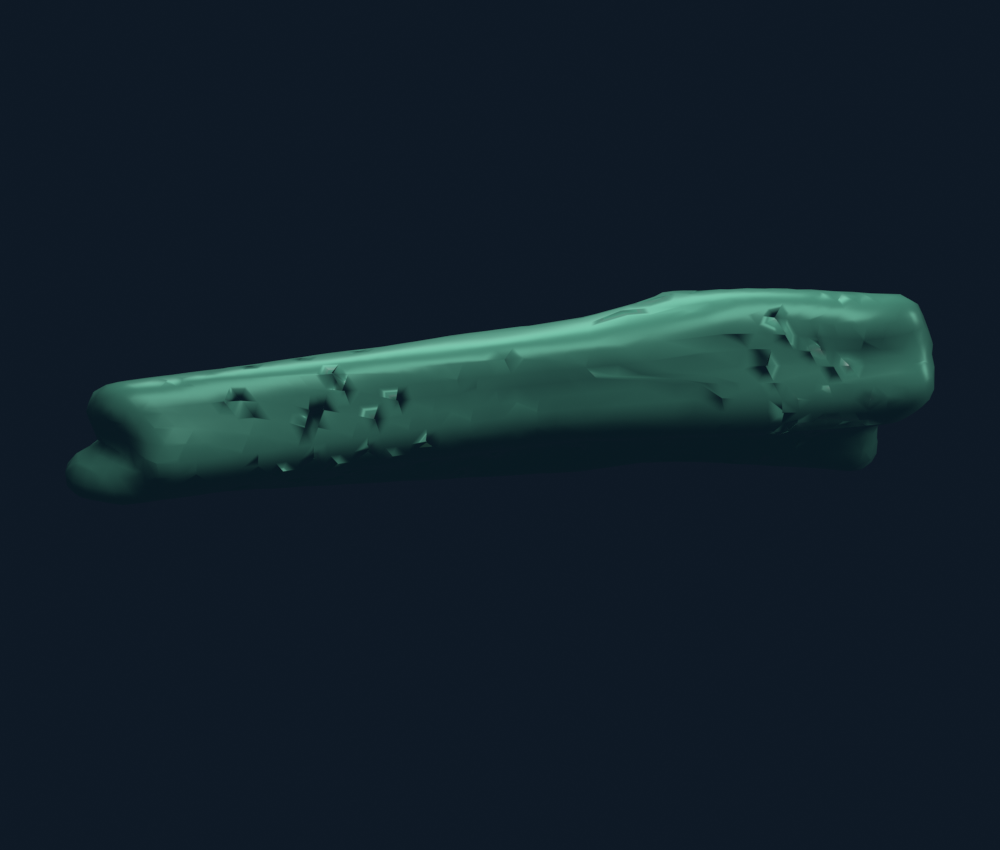
\includegraphics[width=.28\linewidth]{figures/chignolin-phase-0.png}\hfill
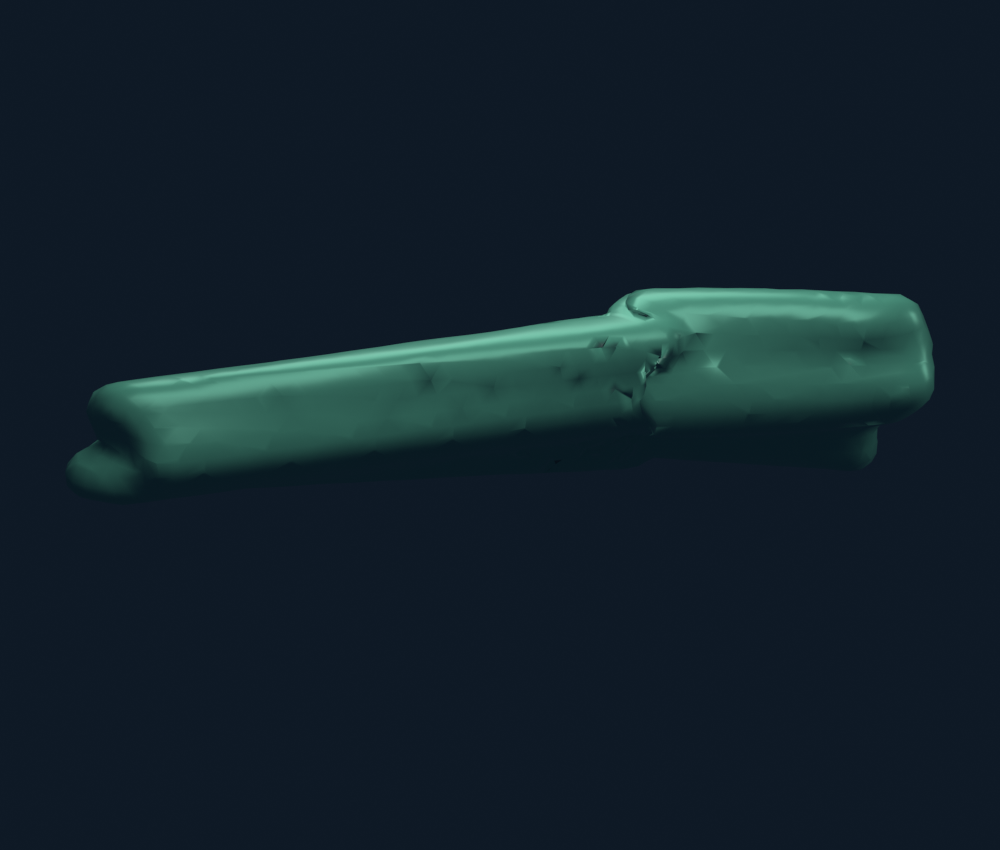
\includegraphics[width=.28\linewidth]{figures/chignolin-phase-1.png}\hfill
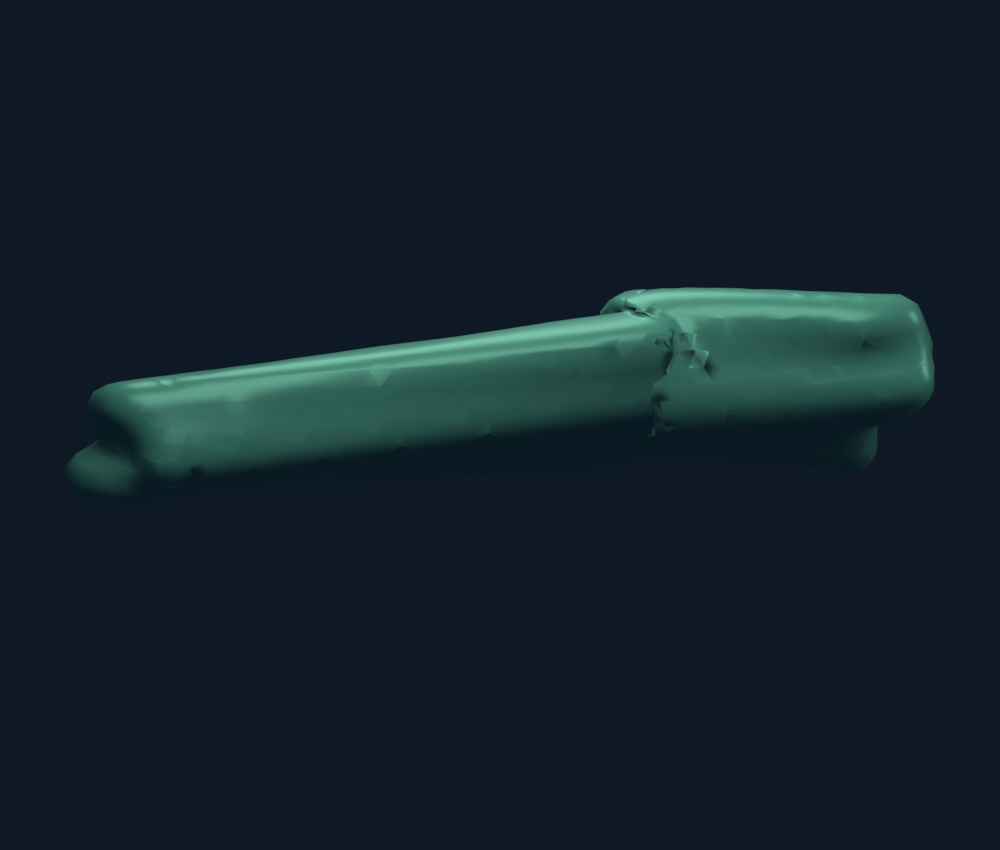
\includegraphics[width=.28\linewidth]{figures/chignolin-phase-2.png}
\caption{\textbf{CLN025 A$\to$C skin at visual phases $0,1/3,2/3$.}
Only this route is shown, under fixed camera and lighting. Surface motion
comes from recorded C$\alpha$ geometry but is not physical time evolution
of a material molecular surface.}
\end{figure}
